\documentclass[letterpaper,10pt]{article}

\usepackage{enumitem}
\usepackage{titling}
\usepackage{listings,listings-rust}
\usepackage{url}
\usepackage{soul}
\usepackage{hyperref}
\usepackage{setspace}
\usepackage{subfig}
\usepackage{sectsty}
\usepackage{pdfpages}
\usepackage{colortbl}
\usepackage{multirow}
\usepackage{multicol}
\usepackage{relsize}
\usepackage{amsmath}
\usepackage{wasysym}
\usepackage{fancyvrb}
\usepackage[yyyymmdd]{datetime}
\usepackage{amsmath,amssymb,amsthm,graphicx,xspace}
\usepackage[titlenotnumbered,noend,noline]{algorithm2e}
\usepackage[compact]{titlesec}
\usepackage{XCharter}
\usepackage[T1]{fontenc}
\usepackage[scaled]{beramono}
\usepackage[normalem]{ulem}
\usepackage{booktabs}
\usepackage{tikz}
\usetikzlibrary{arrows.meta,automata,shapes,trees,matrix,chains,scopes,positioning,calc,decorations.pathreplacing}
\tikzstyle{block} = [rectangle, draw, fill=blue!20, 
    text width=2.5em, text centered, rounded corners, minimum height=2em]
\tikzstyle{bw} = [rectangle, draw, fill=blue!20, 
    text width=4em, text centered, rounded corners, minimum height=2em]

\definecolor{namerow}{cmyk}{.40,.40,.40,.40}
\definecolor{namecol}{cmyk}{.40,.40,.40,.40}
\renewcommand{\dateseparator}{-}

\let\LaTeXtitle\title
\renewcommand{\title}[1]{\LaTeXtitle{\textsf{#1}}}

\lstset{basicstyle=\footnotesize\ttfamily,breaklines=true}

\newcommand{\CPP}{C\nolinebreak\hspace{-.05em}\raisebox{.4ex}{\tiny\bf +}\nolinebreak\hspace{-.10em}\raisebox{.4ex}{\tiny\bf +}}
\def\CPP{{C\nolinebreak[4]\hspace{-.05em}\raisebox{.4ex}{\tiny\bf ++}}}

\newcommand{\handout}[5]{
  \noindent
  \begin{center}
  \framebox{
    \vbox{
      \hbox to 5.78in { {\bf ECE459: Programming for Performance } \hfill #2 }
      \vspace{4mm}
      \hbox to 5.78in { {\Large \hfill #4  \hfill} }
      \vspace{2mm}
      \hbox to 5.78in { {\em #3 \hfill \today} }
    }
  }
  \end{center}
  \vspace*{4mm}
}

\newcommand{\lecture}[3]{\handout{#1}{#2}{#3}{Lecture#1}}
\newcommand{\tuple}[1]{\ensuremath{\left\langle #1 \right\rangle}\xspace}

\addtolength{\oddsidemargin}{-1.000in}
\addtolength{\evensidemargin}{-0.500in}
\addtolength{\textwidth}{2.0in}
\addtolength{\topmargin}{-1.000in}
\addtolength{\textheight}{1.75in}
\addtolength{\parskip}{\baselineskip}
\setlength{\parindent}{0in}
\renewcommand{\baselinestretch}{1.5}
\newcommand{\term}{Winter 2020}

\singlespace


\begin{document}

\lecture{20 --- Performance Case Studies}{\term}{Patrick Lam}

\section*{Making Firefox Fast}

Let's look at Mike Conley's Firefox Performance Updates,
\begin{center}
{\scriptsize
\vspace*{-1em}
\url{https://mikeconley.ca/blog/2018/02/14/firefox-performance-update-1/}
}
\end{center}
\vspace*{-1em}

\begin{itemize}[noitemsep]
\item don't use CPU animating out-of-view elements
\item move db init off main thread
\item keep better profiling data
\item parallel painting for macOS
\item lazily instantiate Search Service only when first search starts
\item halve size of the blocklist
\item refactor to reduce main-thread IO
\item don't hold all frames of animated GIFs/APNGs in memory
\item eliminate an unnecessary hash table
\item use more modern compiler
\end{itemize}

We can categorize most of these updates into the categories we've seen before:
\begin{itemize}[noitemsep]
\item do less work\\
 (or do it sooner/later);
\item use threads (move work off main thread);
\item track performance;
\end{itemize}
Which of the updates fall into which categories?

\subsection*{Tab warming} We continue by examining one particular update, \emph{tab warming}, in detail:
\begin{center}
\scriptsize
\vspace*{-1em}
\url{https://mikeconley.ca/blog/2018/01/11/making-tab-switching-faster-in-firefox-with-tab-warming/}.
\end{center}
\vspace*{-1em}

\hfill ``Maybe this is my Canadian-ness showing, but I like to think of it almost like coming in from shoveling snow off of the driveway, and somebody inside has \emph{already made hot chocolate for you}, because they knew you’d probably be cold.'' --- Mike Conley

Consider switching tabs. Previously, Firefox would request a paint of the newly-selected tab and wait for the rendering to be available before switching the tab.

The idea is to reduce user-visible latency by predicting an imminent tab switch. How do you know that the user is about to switch tabs? When the user has a mouse, then the mouse cursor will hover over the next tab.

\begin{quote}
Assuming a sufficiently long delay between hover and click, the tab switch should be perceived as instantaneous. If the delay was non-zero but still not long enough, we will have nonetheless shaved that time off in eventually presenting the tab to you.

And in the event that we were wrong, and you weren’t interested in seeing the tab, we eventually throw the uploaded layers away.
\end{quote}

The blog post does not report performance numbers (but bug 1430160 discusses how to collect them).

\subsection*{Firefox in general}

Try: ``about:mozilla'' in Firefox. On a Quantum Flow-enabled version, you'll see

\begin{center}
\emph{The Beast adopted new raiment and studied the ways of Time and Space and Light and the Flow of energy through the Universe. From its studies, the Beast fashioned new structures from oxidised metal and proclaimed their glories. And the Beast’s followers rejoiced, finding renewed purpose in these teachings.}

\hfill \emph{from The Book of Mozilla, 11:14}
\end{center}

In 2017, Mozilla released Electrolysis (E10s)~\cite{electrolysis}.
which leverages multicore processors by using multiple OS-level
processes. (Chrome has always done this, but Firefox attempts to also
keep memory usage
down~\cite{goldilocks}.
Beyond internal architecture issues, handling Add-Ons (now
WebExtensions) was perhaps the most challenging part of going
multi-process.

Note the connection to different thread/process models.
Chrome is one-process-per-tab, while Firefox multiplexes tabs across
the 4 content processes (``hardware threads'', by analogy). Limiting
the number of tabs also limits the memory consumption of the browser:
we don't have arbitrary numbers of renderer state.

\begin{center}
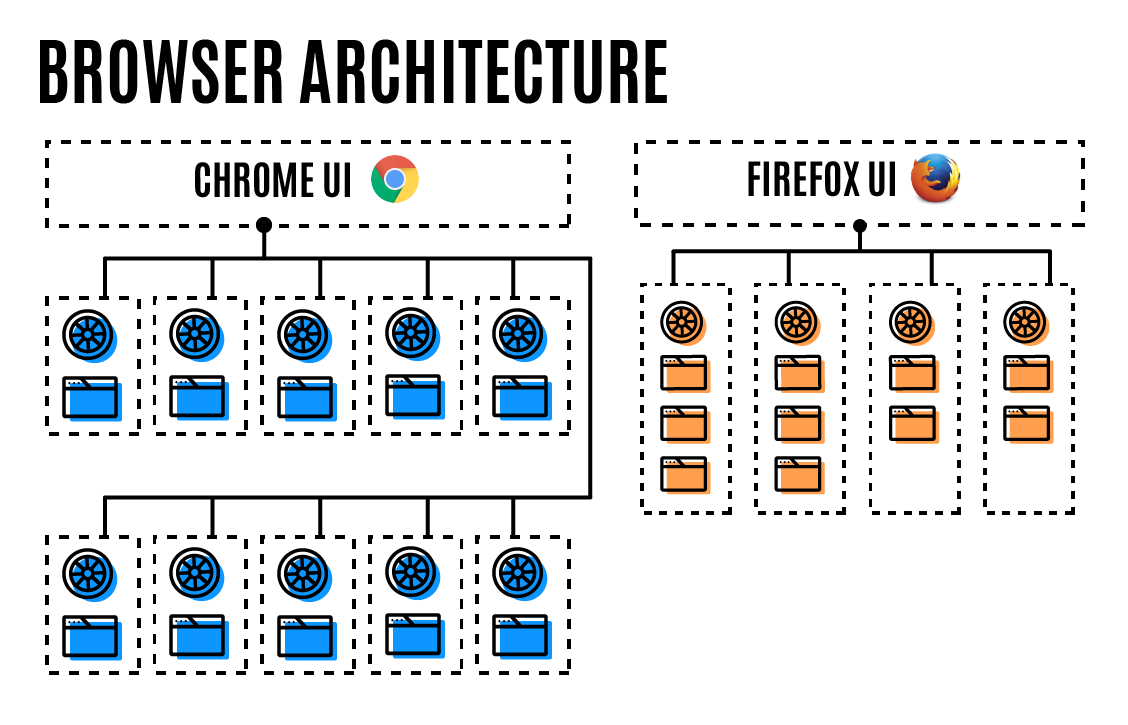
\includegraphics[width=.9\textwidth]{images/L19-chrome-vs-firefox.png}
\end{center}
Source: Ryan Pollock~\cite{goldilocks}

As a crude summary, Electrolysis works on splitting across processes
while the newer Quantum Flow leverages multithreading and other
improvements.  Quantum Flow uses the Rust programming language and its
``fearless concurrency'' (in Rust-speak). Rust should probably be part
of a future revision of the ECE 459 curriculum. But we'll focus on
Firefox here.

\subsection*{Quantum Flow}
Here's a retrospective of the Quantum Flow project:
\begin{center}
\url{https://ehsanakhgari.org/blog/2017-09-21/quantum-flow-engineering-newsletter-25}
\end{center}

To sum up, they formed a small team and did the following.
\begin{enumerate}[noitemsep]
\item Measure slowness: gather information, instrument Firefox, collect profiling data and measurements. Prioritize issues.
\item Gather help: convince other teams to pitch in with perf improvements. Examples: front-end team (reduce flushes, timers); layout team (reflow performance).
\item Fix all the things! (Or at least the most important ones).
\end{enumerate}
Given the short timeline they gave themselves (6 months) and the limited resources, an important part of their work was convincing others to help.
They triaged 895 bugs and fixed 369 of them. The weekly Quantum Flow Engineering Newsletter was a key motivational tool.

After the project wound down, they aimed to distribute responsibility for perf improvements across the entire project.

\section*{Firefox Telemetry}
Firefox's Telemetry feature collects lots of information from Firefox
users.  Idea: collect data before hacking away at things.  Firefox collects hundreds of
gigabytes of anonymous metrics per day while browsing and makes it all available to
the public.  One can view this as an analogy of CPU profiling on a
massively distributed context. This data is collected much less often than
CPU profiling data but at a much broader scope.
\begin{center}
\url{https://telemetry.mozilla.org/}
\end{center}
If you are running Firefox and want to see what it is collecting:
\begin{center}
\url{about:telemetry}
\end{center}

You can view distributions of telemetry probes (in the form of
histograms). You can also make your own dashboard based on Firefox
Telemetry data and Mozilla has infrastructure for their developres to
formulate and evaluate their own queries.

Example questions:
\begin{itemize}[noitemsep]
\item Is Firefox the user's default browser? (69\% yes)
\item Does e10s make startup faster? (no, slower)
\item Which plugins tend to freeze the browser on load? (Silverlight and Flash)
\end{itemize}
Can see evolution of data over time.

Firefox developers can propose new telemetry probes which are reviewed
for data privacy\footnote{Mozilla Data Collection Practices: \url{https://wiki.mozilla.org/Firefox/Data_Collection}} as well as through normal code review channels.

\paragraph{Pings.} Firefox phones the data home using so-called ``pings''.
Firefox sends a ``main ping'' every 24 hours, upon shutdown, environment change,
and crash. There are other types of pings as well. Pings get sent either by Firefox
or by a helper program, Pingsender, when Firefox isn't running. Presumably they
are sent over the network as compressed JSON to a central server.

Here's the common ping structure:

\begin{verbatim}
{
  type: <string>, // "main", "activation", "optout", "saved-session", ...
  id: <UUID>, // a UUID that identifies this ping
  creationDate: <ISO date>, // the date the ping was generated
  version: <number>, // the version of the ping format, currently 4

  application: {
    architecture: <string>, // build architecture, e.g. x86
    buildId: <string>, // "20141126041045"
    name: <string>, // "Firefox"
    version: <string>, // "35.0"
    displayVersion: <string>, // "35.0b3"
    vendor: <string>, // "Mozilla"
    platformVersion: <string>, // "35.0"
    xpcomAbi: <string>, // e.g. "x86-msvc"
    channel: <string>, // "beta"
  },

  clientId: <UUID>, // optional
  environment: { ... }, // optional, not all pings contain the environment
  payload: { ... }, // the actual payload data for this ping type
}
\end{verbatim}

Pings contain scalars (counts, booleans, strings) and histograms. A histogram collects
bucketed data (think grade distributions). Both scalars and histograms can be keyed, e.g.
how often searches happen for which search engines.

\section*{Case Study: Is Lower Level Always Faster?}
There's a lot of support for the idea that code written in lower level languages (e.g., choosing C rather than \CPP) means that your code will be faster. Is that always the case? Language elitism aside -- not always!

    \CPP11 has made major strides towards readability and
    efficiency---it provides light-weight abstractions. We'll look at
    a couple of examples.

\paragraph{Sorting.} Our goal is simple: we'd like to sort a bunch of integers.
In C, you would usually just use qsort from {\tt stdlib.h}.

  \begin{lstlisting}
void qsort (void* base, size_t num, size_t size,
            int (*comparator) (const void*, const void*));
  \end{lstlisting}

This is a fairly ugly definition (as usual, for generic C functions). How ugly is it?
Let's look at a usage example.
  \begin{lstlisting}[language=C]
#include <stdlib.h>

int compare(const void* a, const void* b) {
    return (*((int*)a) - *((int*)b));
}

int main(int argc, char* argv[]) {
    int array[] = {4, 3, 5, 2, 1};
    qsort(array, 5, sizeof(int), compare);
}
  \end{lstlisting}
This looks like a nightmare, and is more likely to have bugs than what we'll see next.


C++ has a sort with a much nicer interface\footnote{\ldots well, nicer to use, after you get over templates.}:

  \begin{lstlisting}[language=C++]
template <class RandomAccessIterator>
void sort (
    RandomAccessIterator first,
    RandomAccessIterator last
);

template <class RandomAccessIterator, class Compare>
void sort (
    RandomAccessIterator first,
    RandomAccessIterator last,
    Compare comp
);
  \end{lstlisting}
It is, in fact, easier to use:
  \begin{lstlisting}[language=C++]
#include <vector>
#include <algorithm>

int main(int argc, char* argv[])
{
    std::vector<int> v = {4, 3, 5, 2, 1};
    std::sort(v.begin(), v.end());
}
  \end{lstlisting}

{\bf Note:} Your compare function can be a function or a functor. (Don't know what functors
are? In C++, they're functions with state.) By default,
  {\tt sort} uses {\tt operator$<$} on the objects being sorted.

  \begin{itemize}
    \item Which is less error prone?
    \item Which is {\bf faster}?
  \end{itemize}

The second question is empirical. Let's see. We generate an array of 2 million ints
and sort it (10 times, taking the average).

\begin{itemize}
\item qsort: 0.49 seconds
\item C++ sort: 0.21 seconds
\end{itemize}

The C++ version is {\bf twice} as fast. Why?
      \begin{itemize}
        \item The C version just operates on memory---it has no clue about the
          data.
        \item We're throwing away useful information about what's being sorted.
        \item A C function-pointer call prevents inlining of the compare function.
      \end{itemize}
OK. What if we write our own sort in C, specialized for the data?

\begin{itemize}
\item Custom C sort: 0.29 seconds
\end{itemize}

Now the C++ version is still faster (but it's close). But, this is
quickly going to become a maintainability nightmare.
      \begin{itemize}
        \item Would you rather read a custom sort or 1 line?
        \item What (who) do you trust more?
      \end{itemize}

\subsection*{Lesson}
Abstractions will not make your program slower. 

\noindent
They allow speedups and are much easier to maintain and read.

\subsection*{Vectors vs Lists}
Consider two
problems.

\begin{enumerate}
\item Generate {\bf N} random integers and insert them into (sorted)
      sequence.
      
      {\bf Example:} 3 4 2 1
      
      \begin{itemize}
        \item 3
        \item 3 4
        \item 2 3 4
        \item 1 2 3 4
      \end{itemize}

\item Remove {\bf N} elements one-at-a-time by going to a random position
      and removing the element.

      {\bf Example:} 2 0 1 0
      
      \begin{itemize}
        \item 1 2 4
        \item 2 4
        \item 2
        \item 
      \end{itemize}
\end{enumerate}

For which {\bf N} is it better to use a list than a vector (or array)?

 
\paragraph{Complexity analysis.} As good computer scientists, let's analyze
the complexity.  

{\bf Vector}:\\[-2em]
      \begin{itemize}
        \item Inserting\\[-2em]
          \begin{itemize}
            \item $O(\log n)$ for binary search
            \item $O(n)$ for insertion (on average, move half the elements)
          \end{itemize}
        \item Removing\\[-2em]
          \begin{itemize}
            \item $O(1)$ for accessing
            \item $O(n)$ for deletion (on average, move half the elements)
          \end{itemize}
      \end{itemize}

{\bf List}:\\[-2em]
      \begin{itemize}
        \item Inserting\\[-2em]
          \begin{itemize}
            \item $O(n)$ for linear search
            \item $O(1)$ for insertion
          \end{itemize}
        \item Removing\\[-2em]
          \begin{itemize}
            \item $O(n)$ for accessing
            \item $O(1)$ for deletion
          \end{itemize}
      \end{itemize}

Therefore, based on their complexity, lists should be better.

\paragraph{Reality.} OK, here's what happens. 
\begin{verbatim}
$ ./vector_vs_list 50000
Test 1
======
vector: insert 0.1s   remove 0.1s   total 0.2s
list:   insert 19.44s   remove 5.93s   total 25.37s
Test 2
======
vector: insert 0.11s   remove 0.11s   total 0.22s
list:   insert 19.7s   remove 5.93s   total 25.63s
Test 3
======
vector: insert 0.11s   remove 0.1s   total 0.21s
list:   insert 19.59s   remove 5.9s   total 25.49s
\end{verbatim}

{\bf Vectors} dominate lists, performance wise. Why?
  \begin{itemize}
    \item Binary search vs. linear search complexity dominates.
    \item Lists use far more memory.
      {\bf On 64 bit machines:}
      \begin{itemize}
        \item Vector: 4 bytes per element.
        \item List: At least 20 bytes per element.
      \end{itemize}
    \item Memory access is slow, and results arrive in blocks:
      \begin{itemize}
        \item Lists' elements are all over memory, hence many
          cache misses.
        \item A cache miss for a vector will bring a lot more usable data.
      \end{itemize}
  \end{itemize}

So, here are some tips for getting better performance.
  \begin{itemize}
    \item Don't store unnecessary data in your program.
    \item Keep your data as compact as possible.
    \item Access memory in a predictable manner.
    \item Use vectors instead of lists by default.
    \item Programming abstractly can save a lot of time.
    \item Often, telling the compiler more gives you better code.
    \item Data structures can be critical, sometimes more than complexity.
    \item {\bf Low-level code != Efficient}.
    \item Think at a low level if you need to optimize anything.
    \item Readable code is good code---different hardware needs different
      optimizations.
  \end{itemize}





\bibliographystyle{alphaurl}
\bibliography{459}


\end{document}
